%%%%%%%%%%%%%%%%%%%%%%%%%%%%%%%%%%%%%%%%%
% Major Acad
% Projects
% Skills
% Courses
% POR
% Extra Curricular
% http://www.LaTeXTemplates.com
%
% Original author:
% Trey Hunner (http://www.treyhunner.com/)
%
% Important note:
% This template requires the resume.cls file to be in the same directory as the
% .tex file. The resume.cls file provides the resume style used for structuring the
% document.
%
%%%%%%%%%%%%%%%%%%%%%%%%%%%%%%%%%%%%%%%%%
%----------------------------------------------------------------------------------------
%	PACKAGES AND OTHER DOCUMENT CONFIGURATIONS
%----------------------------------------------------------------------------------------

\documentclass{report}
\usepackage[utf8]{inputenc}

\title{\textbf{\huge CS 251: Box2D Project Report} \\ \normalsize \emph{ \Large Instructor : Prof. Sharat Chandan } \\ \large Spring 2015}
\author{\Large \textbf{ Author : }Group 25 \\ Sohum Dhar, 140070001 \\ Aakash Praliya , 140050012 \\ Himanshu Payal, 140050011 }


\usepackage[parfill]{parskip} % Do not indent aragraphs
\usepackage{array} % required for boldface tabular columns
\usepackage{ifthen}
\usepackage[left=0.78in,top=0.6in,right=0.78in,bottom=0.6in]{geometry}
\usepackage{multirow}
\usepackage{ragged2e}
\usepackage{natbib}
\usepackage{url}
\usepackage{hyperref}
\usepackage{graphicx}
\usepackage{amssymb}
\usepackage{wrapfig}
\usepackage{float}
%\usepackage{subfigure}
\usepackage{subcaption}
\begin{document}
\maketitle

\renewcommand*\sectionmark[1]{\markboth{#1}{}}
\renewcommand*\subsectionmark[1]{\markright{#1}}
\newcommand{\tab}[2]{\hspace{0em}\rlap{#1}\hspace{0.245\textwidth}\rlap{#2}}
\newenvironment{rSection}[1]
{ \MakeUppercase{\bf \large #1}
  \bigskip  \hrule
  \begin{list}{}{ \setlength{\leftmargin}{1.5em} }
  \item[]
}
{ \end{list}
  \pagebreak}
\newenvironment{rSubsection}[4]{
  %%%%%%%%%%%%%%%%%%%%%% Default Layout: %%%%%%%%%%%%%%%%%%%%%%%%
  %% Employer (bold) Dates (regular) %%
  %% Title (emphasis) Location (emphasis) %%
  %%%%%%%%%%%%%%%%%%%%%%%%%%%%%%%%%%%%%%%%%%%%%%%%%%%%%%%%%%%%%%%
  {\bf #1} \hfill { #2}
  \ifthenelse{\equal{#3}{}}{}{
  \\
  {\em #3} \hfill {\em #4}
  }\smallskip
  % \cdot used for bullets, items non-indented
  \begin{list}{$\cdot$}{\leftmargin=0em}
  \itemsep -0.5em \vspace{-0.5em}
  }{\end{list}
  \vspace{0.5em}
}

\section*{\huge 1. INTRODUCTION}
\hrule
This is the report for CS251 Box2D Project, discussing various aspects of the project. 
\\
\section*{1.1 PURPOSE}
\hrule
\large
\begin{list}{$\cdot$}{\setlength{\leftmargin}{0em}}
\item Motivated by the potential of Box2D platform to develop a simulation of Rube Goldberg Machine, i.e. setting up a simulation of a sequence of connected events to accomplish a simple task. We have developed a fairly complicated simulation for a simple task: "Turning the Fans ON".
\item This project is prepared for CS251 - Software Systems Lab, Instructor: Prof. Sharat Chandan.
\end{list}
\section*{1.2 SCOPE}
\hrule
\large
\begin{list}{$\cdot$}{\setlength{\leftmargin}{0em}}
\item This project, "Get Some Air!", is a simulation of a Rube Goldberg Machine in Box2D physics engine.
\item Once run, the physics engine, Box2D, displays the setting of the simulation and the chain of events begin. In the end, the fan is turned on. 
\item Also, the user can play around with objects in the simulation by clicking and dragging them with the mouse.
\item This project can be extended to be part of some game or other simulation developed on Box2D platform. 
\end{list}
\section*{1.3 OVERVIEW}
\hrule
\large
\begin{list}{$\cdot$}{\setlength{\leftmargin}{0em}}
\item The rest of the report talks about the various aspects, perspectives, functions of the product/project. It also discussing the performance and profiling data of the project during execution.
\item The report discusses the difficulties and challenges faced and the solutions/techniques adopted.
\end{list}

\pagebreak
%-----------------------------------------
%       PRELIMINARY DESIGN SECTION
%-----------------------------------------
\section*{\huge 2. GENERAL DESCRIPTION}
\hrule
This project, "Get Some Air!" is a simulation on Box2D platform, of a Rube Goldberg Machine which turns on fans!
\section*{2.1 PRELIMINARY DESIGN}
\hrule
\large
The following is the prelimanry design fo the Rube Goldberg Machine Design
\begin{figure}[h]
\centering
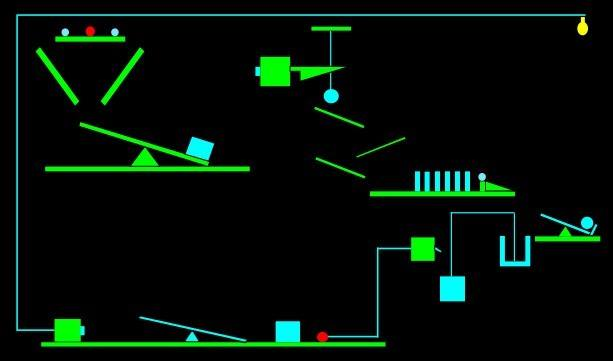
\includegraphics[width=0.75\textwidth]{latex/box2d_prelim.jpg}
\caption{Preliminary Design}
\end{figure}

The preliminary design consists of the following segments/sections.
\begin{enumerate}{\leftmargin=0em}
\item \textbf{The Kick-Off Section} contained an explosive element\cite{explosion}, two balls, redirecting edges, a see saw system and a pushing-box.
This is where the simulation starts! When the bomb explodes, the two spheres are pushed away.They fall down the redirecting edges onto the see saw. The box on the other side is thrown into the air to "pass the baton"...
\item \textbf{The Saw and Dominos Section} contains an oscillating saw \cite{pendulum} (which starts on the push of the button), a suspended ball, a sequense of slopes and series of waiting dominos \cite{dominos}. 
This is an interesting and challenging part of the project where, a saw when switched on cuts the thread and sets off the ball down the slopes.Finally, it hits the dominos and "pass the baton"...
\item \textbf{The See-Saw and Pulley Section} consists of a ball on wedge, a see saw, a pulley element \cite{pulley}.
Remember the above series on (falling) dominos? The last one will tap the ball on top of the wedge. It rolls down the incline on to the see saw. Throwing the weight(ball on other side) into the air. The weight(ball) will fall into the open container of the pulley. The pulley is now unbalanced and so the other side(switching bar) begins to rise.
\item \textbf{The Button Section} This is the finale! Remember the pulley(rising)? The rising bar on left will turn on the switch to set off the detonator. The box down there gets the thrust to slide up the see-saw and hit the button to make fan/light go off.
\end{enumerate}
\pagebreak

%-----------------------------------------
%       Actual Machine Image
%-----------------------------------------
\section*{2.2 PRODUCT/PROJECT OVERVIEW}
\hrule
\large
\begin{list}{$\cdot$}{\leftmargin=0em}
\item The following is the image of the actual implementation.
\begin{figure}[h]%{0.75\textwidth}
\centering
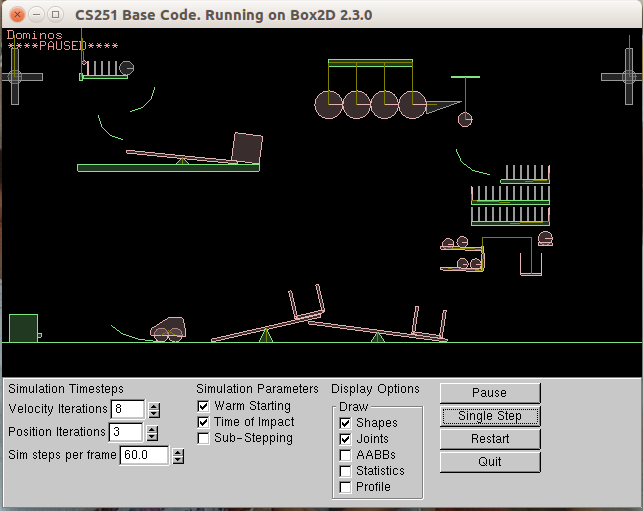
\includegraphics[width=0.75\textwidth, width=0.65\textwidth]{latex/box2d_prelim2.png}%final.jpg}
\caption{Box2D Project Image}
\end{figure}
\begin{figure}
\begin{subfigure}[h]{0.3\textwidth}
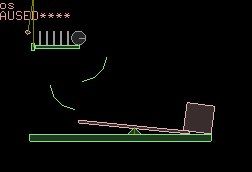
\includegraphics[width=\textwidth, height=0.5\textwidth]{latex/box2d_1.png}
\caption{Kick-Off}
\end{subfigure}
\begin{subfigure}[h]{0.3\textwidth}
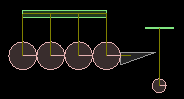
\includegraphics[width=\textwidth, height=0.5\textwidth]{latex/box2d_2.png}
\caption{Pendulems and Saw}
\end{subfigure}
\begin{subfigure}[h]{0.3\textwidth}
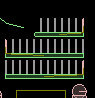
\includegraphics[width=\textwidth, height=0.5\textwidth]{latex/box2d_3.png}
\caption{Three Planks}
\end{subfigure}
\centering
\begin{subfigure}[h]{0.3\textwidth}
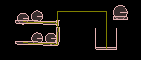
\includegraphics[width=\textwidth, height=0.5\textwidth]{latex/box2d_4.png}
\caption{Loaded Pulley}
\end{subfigure}
\begin{subfigure}[h]{0.3\textwidth}
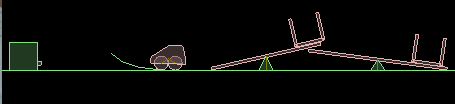
\includegraphics[width=\textwidth, height=0.5\textwidth]{latex/box2d_5.png}
\caption{Finale}
\end{subfigure}
\end{figure}

\end{list}
\pagebreak

%-----------------------------------------
%       Actual Machine Internals
%-----------------------------------------

\section*{2.3 PRODUCT/PROJECT FUNCTIONS}
\hrule
\large
\emph{The product/project is a Box2D simulation of a Rube Goldberg Machine. Product/Project's design implementation consists of the following segments/sections explained in detail.}\\
\begin{wrapfigure}{r}{0.32\textwidth}
\begin{center}
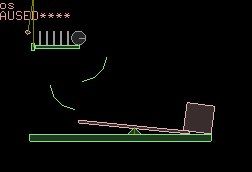
\includegraphics[width=0.3\textwidth, height=0.2\textwidth]{latex/box2d_1.png}
\end{center}
\caption{Machine Internals(MI): Kick-Off}\vspace{-10pt}
\end{wrapfigure}
\textbf{2.3.1. THE KICK OFF SECTION}
\begin{list}{$\cdot$}{\setlength{\leftmargin}{0em}}
\item Contains \textbf{a pendulum\cite{pendulum}, a series of dominos\cite{dominos}, a heavy ball}, \textbf{redirecting edges, see-saw, light box}.
\item The pendulum swings down to hit the leftmost domino. Thus, the series of dominos fall one by one(well, they are dominos!) and the last domino taps the heavy sphere. The sphere falls down, on  the redirecting edges and on to the see-saw. Well, it's heavy so it disrupts the balance and throws the light box into the air. Then it rolls down the see-saw and falls deep down into a container, waiting... 
\item \emph{The \textbf{explosion\cite{explosion} kick} is replaced by the \textbf{pendulum and the series of dominos setting}. The pendulum gives the push instead of the explosive element.}\\
\end{list}


\begin{wrapfigure}{r}{0.32\textwidth}
\begin{center}
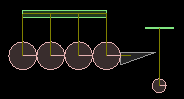
\includegraphics[width=0.3\textwidth, height=0.2\textwidth]{latex/box2d_2.png}
\end{center}
\caption{MI: Dominos and Saw}
\end{wrapfigure}
\textbf{2.3.2. PENDULUMS, SAW AND  BALL SECTION}
\begin{list}{$\cdot$}{\setlength{\leftmargin}{0em}}
\item This section contains a \textbf{ series of pendulums \cite{pendulum}, a saw \cite{motor_joint}, a suspended ball \cite{contact_listener}.} 
\item Remember the box thrown into the air? That box pushes the leftmost pendulum in the series. These pendulums swing together and push the saw on right. The saw cuts the thread of the ball. The suspended ball then falls and is redirected ...
\item \emph{The \textbf{button} is replaced by a \textbf{series of pendulums}, just to \textbf{make it more physical than automated}. We have \textbf{kept button for the fans}(in finale).}\\
\end{list}

\begin{wrapfigure}{r}{0.32\textwidth}
\begin{center}
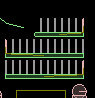
\includegraphics[width=0.3\textwidth, height=0.2\textwidth]{latex/box2d_3.png}
\end{center}
\caption{MI: Three Planks}
\vspace{-10pt}
\end{wrapfigure}
\textbf{2.3.3. THREE PLANKS AND DOMINOS SECTION}
\begin{list}{$\cdot$}{\setlength{\leftmargin}{0em}}
\item This section consists of \textbf{three planks with dominos\cite{dominos} on them, a revolvable platform \cite{revolute_joint} and a heavy sphere.}
\item Remember the above ball(falling)? It falls down on the redirecting edges, on to the top plank, hitting leftmost domino. The series of dominos fall one by one(as they are dominos). The last domino is hinged\cite{revolute_joint} at its base with the plank. It makes a 180 degree rotation and hits the domino below. This cycle goes on till the third plank. The last domino of the third plank taps the sphere on the revolvable platform. The platform is then imbalanced and the heavy sphere falls down.
\item \emph{We have upgraded the proposal by replacing a \textbf{series of dominos} by \textbf{3 planks with 3 series of dominons, where 3 dominos are hinged}.}
\end{list}

\pagebreak

\begin{wrapfigure}{r}{0.32\textwidth}
\begin{center}
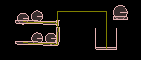
\includegraphics[width=0.3\textwidth, height=0.2\textwidth]{latex/box2d_4.png}
\end{center}
\caption{MI: Loader Pulley}
\end{wrapfigure}
\textbf{2.3.4. LOADER PULLEY SECTION}
\begin{list}{$\cdot$}{\setlength{\leftmargin}{0em}}
\item This section contains a \textbf{pulley\cite{pulley} formed by an open container and a loader\cite{revolute_joint} with 4 heavy balls on the other side}.
\item Recall the sphere falling (above). This sphere is caught by the open box on right, imbalancing the pulley. Thus, the loader on the left if pulled up from right(note that the loader's left ends are hinged). The balls(2 on each level) start to roll down. Since the friction on the lower level is more than that on the upper level, the balls on the upper level fall before those on the lower level. They are collected into the container below, on right. 
\item \emph{We have replaced the previous \textbf{simple pulley, see saw system} with a fairly complicated module of \textbf{"loader-pulley system"}.}\\
\end{list}

\begin{wrapfigure}{r}{0.32\textwidth}
\begin{center}
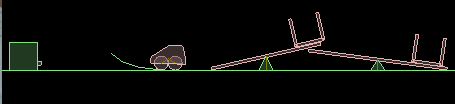
\includegraphics[width=0.3\textwidth, height=0.2\textwidth]{latex/box2d_5.png}
\end{center}
\caption{MI: Series of See Saws}
\end{wrapfigure}
\textbf{2.3.5. FINALE}
\begin{list}{$\cdot$}{\setlength{\leftmargin}{0em}}
\item This section consists of \textbf{two back to back see-saws \cite{revolute_joint} with containers on right and the magic fans' button \cite{contact_listener}!}
\item is the finale! Recall the heavy shere from first section that had fallen into the left container below. Also recall the heavy spheres were falling from the loader(above). As these spheres fall into the right container, the left container is thrown into the air. It then topples to the left and descends. Finally the ball rolls to the left and pushes the car. The car jumps over the ramp and touches the switch \cite{contact_listener} and CONGRATS the fan are turned on! We can finally have some cool air!
\item \emph{The \textbf{explosion element} is replaced by \textbf{the series of see-saws}. It was difficult to make the ball go to the right. We have tried to \textbf{compensate the explosion element by the timing, complexity and excitement of the see-saw series system. Plus we have added a car jumping over a ramp}}  
\end{list}

\section*{2.4 USER CHARECTERSTICS}
\hrule \large
\begin{list}{$\cdot$}{\setlength{\leftmargin}{0em}}
\item The user is expected to use the makefile, i.e. command-line to compile and run the project/product.
\item During the run of the program the user should not click or drag any of the objects in the simulation. Also the user must not change settings of the interface (Velocity Iterations, Sim step per frame, Position Iterations).
\end{list}

\section*{2.5 ASSUMPTIONS AND DEPENDEDENCIES}
\hrule \large
\begin{list}{$\cdot$}{\setlength{\leftmargin}{0em}}
\item We have developed the simulation for specified values of "Velocity Iterations", "Sim step per frame", "Position Iterations", i.e. 8, 60.0, 3 respectively.
\item It is assumed that the simulation does not slow down too much during the run(so that timings within the simulation are not deviated a lot).
\end{list}

\section*{2.6 CONTRIBUTION}
\hrule \Large
\begin{tabular}{@{} >{\bfseries}l @ {\hspace{5.0ex}} l @{}>{\bfseries}l  }
Himanshu Payal & Project ideation (main), Explosion element,&\\& Base Code, Web Page & 100\%\\
Aakash Praliya & Fan button, Thread Cutting(Contact Listener),& \\ &  Base Code, Project Ideation, Makefile& 100 \% \\
Sohum Dhar &  Base Code(main), Report, Documentation(main), & \\ & Makefile(main), Presentation, Project Ideation & 100\%\\  
\end{tabular}

\section*{2.7 DIFFICULTIES FACED AND TECHNIQUES/SOLUTIONS USED}
\hrule \large
\begin{list}{$\cdot$}{\setlength{\leftmargin}{0em}}
\item The challenges in this project were:
\textbf{
\begin{enumerate}
\item Getting the Timing right
\item Making the Saw cut the Thread
\item Making switch (for the Fans(finale) etc.)
\item Making Car element
\item Creating Explosive Elements
\item Making the Objects Move with the Mouse!
\end{enumerate}}
\item We \textbf{got the timings right} by setting the densities, friction etc. of various elements in the simulation(\textbf{trial and error technique} learnt in lab03). Also, getting the timing right especially \textbf{for the loader element}. For example, if the lower balls fall first the sphere in the container would go to the right instead of left! We used \textbf{logic and trial and error method}(lab03) for solving this.
\item To \textbf{make the saw cut the thread} and to \textbf{make the switch} we needed to learn about \textbf{Contact Listeners} \cite{contact_listener} 
\item To make the car element \cite{test_bed} of appropriate dimension and weight, it took a while. The car won't become stable! It would jump on and on and disrupt the simulation!
\item We used concepts learnt in \textbf{Lab02} to make the \textbf{WebPage}! 
\item We used concepts learnt in \textbf{Lab05} to make the \textbf{Makefile}!
\item We used \textbf{Beamer} and\textbf{\LaTeX} (as learnt in \textbf{Lab06}) to create the presentation and this report!
\item We used the \textbf{gprof}\cite{gprof} feature(as learnt in \textbf{Lab09}) to profile the code, for performance report and improvisation-making code efficient(as learnt in Lab09).
\item Due to pausity of time we were unable to finish the explosion element. However we have added an additional feature \cite{test_bed} where the user can move things around by \textbf{dragging and dropping with mouse!}
\item We also have tried to improve \textbf{graphics }\cite{openGL}  by making changes in the render.cpp file.
\end{list}
\pagebreak
\section*{\huge 3. SPECIFIC REQUIREMENTS}
\hrule \large
In this section we discuss some D-requirements of the project. For the complete guide to D-requirements, project's software design and implementation one can refer to project-documentation.

\section*{3.1 EXTERNAL INTERFACE REQUIREMENTS}
\large \textbf{3.1.1 USER INTERFACES}
\begin{list}{$\cdot$}{\setlength{\leftmargin}{0em}}
\item The user interaction with the program is one of observation till the simulationends. Later the user can play around with he objects in the simulation- click and drag them around.
\end{list}

\large \textbf{3.1.2 HARDWARE INTERFACES}
\begin{list}{$\cdot$}{\setlength{\leftmargin}{0em}}
\item This project does not require any special external hardware.
\item The project responds/interacts with the mouse(click and drag).
One can also change the settings displayed in the GUI with keyboard, mouse(select, check).
\end{list}

\large \textbf{3.1.3 SOFTWARE INTERFACES}
\begin{list}{$\cdot$}{\setlength{\leftmargin}{0em}}
\item The project can only be run on a linux-based OS. This is the requirement of the Box2D(Linux) platform used.
\item The project uses C++, openGL, glut, libgdx, freeglut, Box2D for implementation.
\end{list}

\section*{3.2 FUNCTIONAL REQUIREMENTS}
\hrule \large Discussed in project documentation.

\section*{3.5 NON FUNCTIONAL REQUIREMENTS}

\large \textbf{3.5.1 PERFORMANCE}
\begin{list}{$\cdot$}{\setlength{\leftmargin}{0em}}
\item Performance is analysed using gprof \cite{gprof}.
\item This analysis is discussed in Section 4.1. 
\end{list}

\large \textbf{3.5.2 AVAILABILITY}\\
The project is publically available on github.

\large \textbf{3.5.3 PORTABILITY}\\
Portable to any Linux-based OS.

\section*{3.6 DESIGN CONSTRAINTS}
\hrule \large
\begin{list}{$\cdot$}{\setlength{\leftmargin}{0em}}
\item The simulation is developed in 2D
\item The number of elements is $\geq$ 10
\end{list}
%----------------------------------------------------------------------------------------
%	GPROF DATA SECTION
%-----------------------------------------------------------------------------------
\begin{figure}[b]
\huge 4. ANALYSIS MODELS \\
\hrule \large
Analysis of the project is done using 'gprof' \cite{gprof} functionality. 
\section*{4.1 PROFILING PLOTS AND DATA \\}
\hrule
\large Analysing data after 100, 500, 1000, 2500 iterations, we get the following data, represented pictorially,

\Large \begin{center}100 Iterations \hrule \end{center}
\begin{subfigure}[h]{\textwidth}
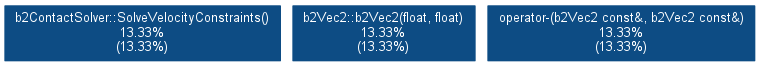
\includegraphics[width=\textwidth, height=0.1\textwidth]{gprof/100_1.png}
\caption{}
\end{subfigure}
\begin{subfigure}[h]{\textwidth}
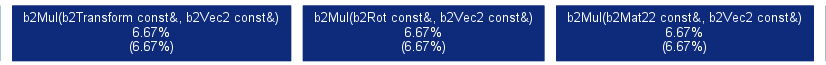
\includegraphics[width=\textwidth, height=0.1\textwidth]{gprof/100_2.png}
\caption{}
\end{subfigure}
\begin{subfigure}[h]{\textwidth}
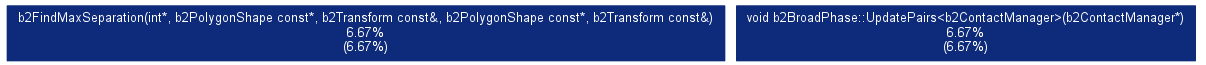
\includegraphics[width=\textwidth, height=0.1\textwidth]{gprof/100_3.png}
\caption{}
\end{subfigure}
\end{figure}s
\begin{figure}
\Large \begin{center}500 Iterations \hrule \end{center}
\begin{subfigure}[h]{\textwidth}
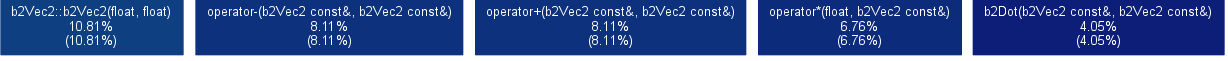
\includegraphics[width=\textwidth, height=0.1\textwidth]{gprof/500_1.png}
\caption{}
\end{subfigure}
\begin{subfigure}[h]{\textwidth}
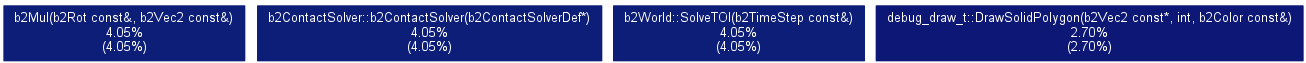
\includegraphics[width=\textwidth, height=0.1\textwidth]{gprof/500_2.png}
\caption{}
\end{subfigure}
\begin{subfigure}[h]{\textwidth}
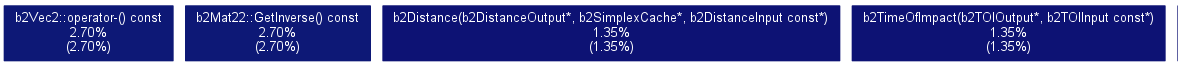
\includegraphics[width=\textwidth, height=0.1\textwidth]{gprof/500_3.png}
\caption{}
\end{subfigure}
\end{figure}
\begin{figure}
\Large \begin{center}2500 Iterations \hrule \end{center}
\begin{subfigure}[h]{\textwidth}
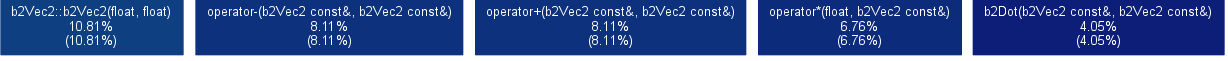
\includegraphics[width=\textwidth, height=0.1\textwidth]{gprof/500_1.png}
\caption{}
\end{subfigure}
\begin{subfigure}[h]{\textwidth}
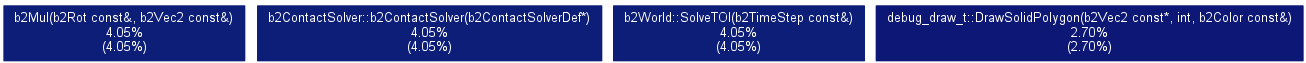
\includegraphics[width=\textwidth, height=0.1\textwidth]{gprof/500_2.png}
\caption{}
\end{subfigure}
\begin{subfigure}[h]{\textwidth}
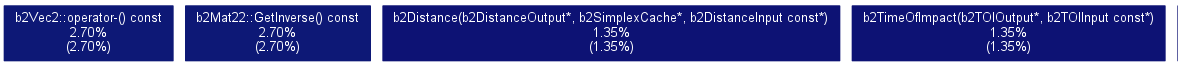
\includegraphics[width=\textwidth, height=0.1\textwidth]{gprof/500_3.png}
\caption{}
\end{subfigure}
\begin{subfigure}[h]{\textwidth}
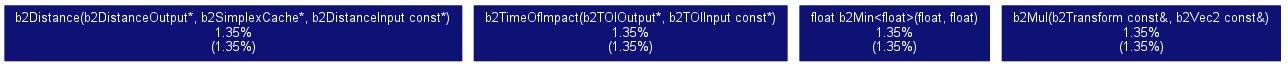
\includegraphics[width=\textwidth, height=0.1\textwidth]{gprof/500_4.png}
\caption{}
\end{subfigure}
\end{figure}
\begin{figure}
\Large \begin{center}3000 Iterations \hrule \end{center}
\begin{subfigure}[h]{\textwidth}
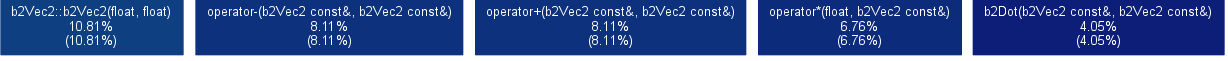
\includegraphics[width=\textwidth, height=0.1\textwidth]{gprof/500_1.png}
\caption{}
\end{subfigure}
\begin{subfigure}[h]{\textwidth}
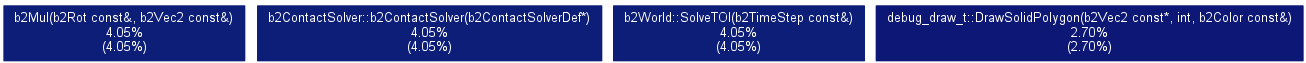
\includegraphics[width=\textwidth, height=0.1\textwidth]{gprof/500_2.png}
\caption{}
\end{subfigure}
\begin{subfigure}[h]{\textwidth}
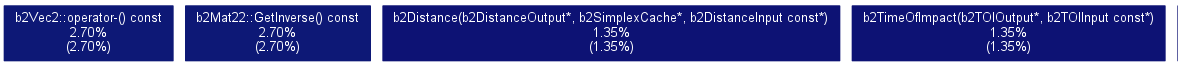
\includegraphics[width=\textwidth, height=0.1\textwidth]{gprof/500_3.png}
\caption{}
\end{subfigure}
\begin{subfigure}[h]{\textwidth}
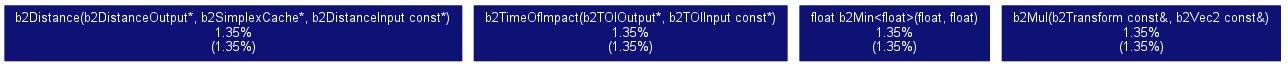
\includegraphics[width=\textwidth, height=0.1\textwidth]{gprof/500_4.png}
\caption{}
\end{subfigure}
\begin{list}{$\cdot$}{}
\item In the original(supplied) base code \emph{b2ContactSolver::SolveVelocityConstraints(), b2World::Solve(), b2World::DrawShape() } take maximum time\textbf{(18.75\%)} followed by \emph{b2ContactManager::Collide()} which takes \textbf{12.5\%} of time. This is because the base code has only simple elements which collide, roll on etc. to complete the chain of events.
\item For this project, operator*() takes maximum time(\textbf{11.13\%}), followed by \emph{operator-()} which takes(\textbf{9.4\%}), followed by \emph{b2ContactSolver::SolveVelocity()} which takes \textbf{7.42\%.} \emph{b2Vec2::b2Vec2()} takes \textbf{6.89\%} and \emph{b2Mul()} takes \textbf{5.43\%.}
\item This is because we have created Contact listeners which reqires b2ContactSolver. Also more number of elements lead to more contacts, collisions which reqire b2ContactSolver. We have created and maintained b2MouseJoint object which require operators on b2Vec2, whose percentage time has increased dramatically! 
\item 
\end{list}
\end{figure}

\pagebreak

%----------------------------------------------------------------------------------------
%	REFERENCES
%----------------------------------------------------------------------------------------

\bibliographystyle{unsrt}
\bibliography{report}
\end{document}
